\chapter{Cloud Environment Evidence}
\label{app:cloud}

This appendix reproduces the Huawei Cloud console views that document the access and network controls of the infrastructure hosting the monitoring and ARIA stack during the internship. They complement the ECS and VPC views already shown in Chapter~2 (Figures~\ref{fig:cloud-ecs}--\ref{fig:cloud-vpc}) and the deployment architecture of Chapter~5. Console URL parameters, agency identifiers, and resource UUIDs have been trimmed or masked; no secret, password, or private key is shown. The hosting network is \codepath{vpc-Smart_Edu} with the \codepath{Smart_edu} subnet (\codepath{10.175.1.0/24}).

\begin{figure}[H]
\centering
\fbox{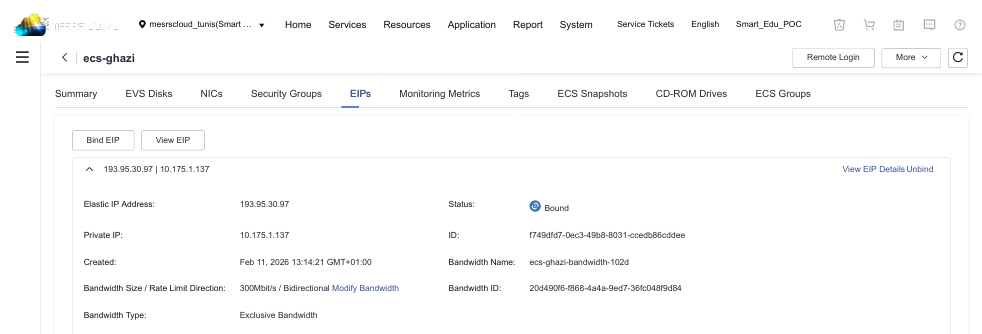
\includegraphics[width=0.96\textwidth,height=0.30\textheight,keepaspectratio]{assets/cloud/cloud_eip.png}}
\caption{Elastic IP bound to the ECS host (public \codepath{193.95.30.97}, private \codepath{10.175.1.137})}
\end{figure}

\begin{figure}[H]
\centering
\fbox{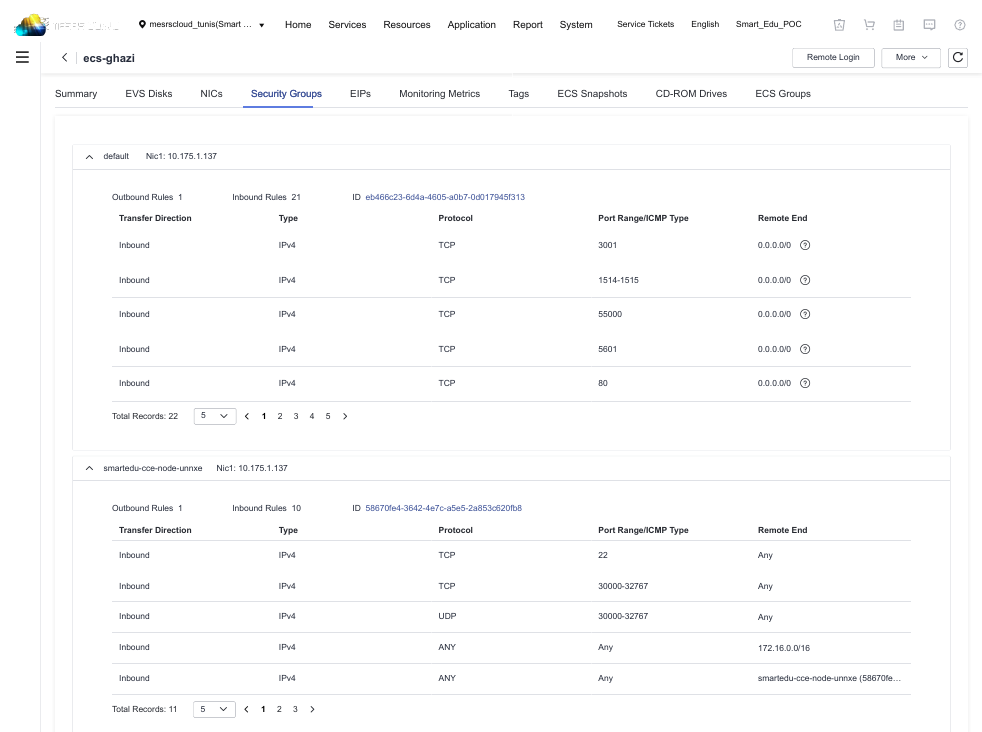
\includegraphics[width=0.96\textwidth,height=0.40\textheight,keepaspectratio]{assets/cloud/cloud_secgroup.png}}
\caption{Security-group rules controlling inbound and outbound access to the SOC host}
\end{figure}

The security group is the main network control between the public Elastic IP and the internal services. As captured here, several inbound rules (for example Kibana on 5601, the Wazuh ports 1514--1515 and 55000, the frontend on 3001, and HTTP on 80) were opened to \codepath{0.0.0.0/0} during internship testing. This was acceptable for an isolated lab but must be restricted before production: only the strictly required ports should be open, administrative access should be limited to trusted networks or a VPN, and Elasticsearch and Redis should never be exposed directly to the public internet.
